%% For double-blind review submission, w/o CCS and ACM Reference (max submission space)
\documentclass[sigplan,review,anonymous]{acmart}\settopmatter{printfolios=true,printccs=false,printacmref=false}
%% For double-blind review submission, w/ CCS and ACM Reference
%\documentclass[sigplan,review,anonymous]{acmart}\settopmatter{printfolios=true}
%% For single-blind review submission, w/o CCS and ACM Reference (max submission space)
%\documentclass[sigplan,review]{acmart}\settopmatter{printfolios=true,printccs=false,printacmref=false}
%% For single-blind review submission, w/ CCS and ACM Reference
%\documentclass[sigplan,review]{acmart}\settopmatter{printfolios=true}
%% For final camera-ready submission, w/ required CCS and ACM Reference
%\documentclass[sigplan]{acmart}\settopmatter{}


%% Conference information
%% Supplied to authors by publisher for camera-ready submission;
%% use defaults for review submission.
\acmConference[ICFP'19]{ACM SIGPLAN International Conference on Functional Programming}{August 18--23, 2019}{Berlin, Germany}
\acmYear{2019}
\acmISBN{} % \acmISBN{978-x-xxxx-xxxx-x/YY/MM}
\acmDOI{} % \acmDOI{10.1145/nnnnnnn.nnnnnnn}
\startPage{1}

%% Copyright information
%% Supplied to authors (based on authors' rights management selection;
%% see authors.acm.org) by publisher for camera-ready submission;
%% use 'none' for review submission.
\setcopyright{none}
%\setcopyright{acmcopyright}
%\setcopyright{acmlicensed}
%\setcopyright{rightsretained}
%\copyrightyear{2018}           %% If different from \acmYear

%% Bibliography style
\bibliographystyle{ACM-Reference-Format}
%% Citation style
%\citestyle{acmauthoryear}  %% For author/year citations
%\citestyle{acmnumeric}     %% For numeric citations
%\setcitestyle{nosort}      %% With 'acmnumeric', to disable automatic
                            %% sorting of references within a single citation;
                            %% e.g., \cite{Smith99,Carpenter05,Baker12}
                            %% rendered as [14,5,2] rather than [2,5,14].
%\setcitesyle{nocompress}   %% With 'acmnumeric', to disable automatic
                            %% compression of sequential references within a
                            %% single citation;
                            %% e.g., \cite{Baker12,Baker14,Baker16}
                            %% rendered as [2,3,4] rather than [2-4].


%%%%%%%%%%%%%%%%%%%%%%%%%%%%%%%%%%%%%%%%%%%%%%%%%%%%%%%%%%%%%%%%%%%%%%
%% Note: Authors migrating a paper from traditional SIGPLAN
%% proceedings format to PACMPL format must update the
%% '\documentclass' and topmatter commands above; see
%% 'acmart-pacmpl-template.tex'.
%%%%%%%%%%%%%%%%%%%%%%%%%%%%%%%%%%%%%%%%%%%%%%%%%%%%%%%%%%%%%%%%%%%%%%


%% Some recommended packages.
\usepackage{booktabs}   %% For formal tables:
                        %% http://ctan.org/pkg/booktabs
\usepackage{subcaption} %% For complex figures with subfigures/subcaptions
                        %% http://ctan.org/pkg/subcaption

\usepackage{listings}
\lstset{ language=haskell%
       , columns=flexible }

\begin{document}

%% Title information
\title[Lazy Infinite Wavelet Expansion]
      {Lazy Evaluation in Infinite-Dimensional Function Spaces with Wavelet Basis}


%% Author information
%% Contents and number of authors suppressed with 'anonymous'.
%% Each author should be introduced by \author, followed by
%% \authornote (optional), \orcid (optional), \affiliation, and
%% \email.
%% An author may have multiple affiliations and/or emails; repeat the
%% appropriate command.
%% Many elements are not rendered, but should be provided for metadata
%% extraction tools.

%% Author with two affiliations and emails.
\author{Olivier Verdier}
\authornote{with author2 note}          %% \authornote is optional;
                                        %% can be repeated if necessary
\orcid{nnnn-nnnn-nnnn-nnnn}             %% \orcid is optional
\affiliation{
  \position{Position2a}
  \department{Department2a}             %% \department is recommended
  \institution{Institution2a}           %% \institution is required
  \streetaddress{Street2a Address2a}
  \city{City2a}
  \state{State2a}
  \postcode{Post-Code2a}
  \country{Country2a}                   %% \country is recommended
}
\email{first2.last2@inst2a.com}         %% \email is recommended
\affiliation{
  \position{Position2b}
  \department{Department2b}             %% \department is recommended
  \institution{Institution2b}           %% \institution is required
  \streetaddress{Street3b Address2b}
  \city{City2b}
  \state{State2b}
  \postcode{Post-Code2b}
  \country{Country2b}                   %% \country is recommended
}
\email{first2.last2@inst2b.org}         %% \email is recommended

\author{Justus Sagemüller}
\affiliation{
  \department{Faculty of Engineering and Science}
  \institution{Høgskulen på Vestlandet}
  \streetaddress{Inndalsveien 28}
  \city{Bergen}
  \state{Hordaland}
  \postcode{5020}
  \country{Norway}
}
\email{mailto_js@gmx.de}


%% Abstract
%% Note: \begin{abstract}...\end{abstract} environment must come
%% before \maketitle command
\begin{abstract}
What is in numerics represented with “vectors” in form of arrays of numbers are often conceptually continuous functions, i.e. elements of a function vector-space.
It would be desirable to express this explicitly with types in the numerical code. A naïve reason why this is normally not done is that the function spaces are infinite-dimensional, whereas the numerical code must run in finite time and memory.

We argue that this is not a hurdle: even in an infinite-dimensional space, the vectors \emph{can} in practice be stored in finite memory. What does require infinite data structures for doing linear algebra are actually just \emph{dual vectors}, also called \emph{distributions}.
Those happen to be equivalent to vectors in the finite-dimensional case, which is why the distinction is usually blurred; but as we show an explicit type-level distinction between functions and distributions makes sense and allows directly expressing useful concepts such as the Dirac distribution, which are problematic in the standard finite-resolution picture.

The example implementation uses a very simple local basis that corresponds to a Haar Wavelet transform.
\end{abstract}


%% 2012 ACM Computing Classification System (CSS) concepts
%% Generate at 'http://dl.acm.org/ccs/ccs.cfm'.
\begin{CCSXML}
<ccs2012>
<concept>
<concept_id>10011007.10011006.10011008</concept_id>
<concept_desc>Software and its engineering~General programming languages</concept_desc>
<concept_significance>500</concept_significance>
</concept>
<concept>
<concept_id>10003456.10003457.10003521.10003525</concept_id>
<concept_desc>Social and professional topics~History of programming languages</concept_desc>
<concept_significance>300</concept_significance>
</concept>
</ccs2012>
\end{CCSXML}

\ccsdesc[500]{Software and its engineering~General programming languages}
\ccsdesc[300]{Social and professional topics~History of programming languages}
%% End of generated code


%% Keywords
%% comma separated list
\keywords{keyword1, keyword2, keyword3}  %% \keywords are mandatory in final camera-ready submission


%% \maketitle
%% Note: \maketitle command must come after title commands, author
%% commands, abstract environment, Computing Classification System
%% environment and commands, and keywords command.
\maketitle


\section{Introduction}

Consider the unit interval $D^1 = [-1,1] \subset \mathbb{R}$. This paper discusses functions on that domain, but the methods have been selected with thought to generalisation to unbounded multidimensional domains in mind.

The set of functions $D^1 \to \mathbb{R}$ is a vector space, but it is not only infinite- but even uncountably-dimensional, which makes any storing of coefficients -- i.e., of discrete function values in the continuous domain -- impractical indeed.
Fortunately, any subset of $\mathbb{R}^{D^1}$ which is closed under scaling and addition is a subspace. Well-studied examples include
\begin{itemize}
 \item $\mathcal{C}^0(D^1)$: continuous functions. These can be characterised thus: to obtain any function value $f(x)$ with at least precision $\varepsilon$, one can instead consider $f(\tilde{x})$ where $\tilde{x}$ needs to be merely \emph{close enough} to $x$, i.e. within a distance $\delta_{x,\varepsilon}$.
 \item $\mathcal{C}^1(D^1)$: continuously differentiable functions. % Discuss how this essentially means just there's a more efficient finite-basis-approximation opportunity
 \item $\mathcal{L}^2(D^1)$: square-integrable functions. % Integral definition
\end{itemize}
Continuity has a straightforward physical interpretation. It can be argued that a function on a non-discrete domain \emph{must} be continuous, at least almost everywhere,
if its values are supposed to be measurable: if it were not, then one would need to set up $x$ exactly before measuring $f(x)$ even approximately, but a physical setup can never be completely exact.
% Contrast with 𝓛² Hilbert space, why that is often preferred in practice, Riesz representation theorem, Nyquist reduction to finite sampling

\section{The space of PCM-sampled functions}
% Discuss standard approach – pre-select, fixed resolution finite-dim space – problem: risk of underestimating required reso or else wasting resources on unnecessary reso
It is possible to have an indeed infinite-dimensional vector-space type approximating $\mathcal{L}^2(D^1)$, with a PCM representation but the choice of a resolution deferred to runtime. The data structure itself is then simply an array (or list) of unspecified finite length $n$,
\begin{lstlisting}
newtype PCM_D¹ y = PCM_D¹ {
          getPCMSampling :: [y] }
\end{lstlisting}
where the \lstinline`y` values correspond to equally-spaced samples of the represented function, i.e.
\[
  \left[f(-1 + \tfrac2n\cdot i)\ \middle|\ i\leftarrow[\tfrac12\;..\;n-\tfrac12]\right].
\]
A harmless, but insightful difficulty with this approach is that vector addition does \emph{not} simply reduce to component-wise addition anymore.
% Demonstrate code&example for `instance AdditiveGroup PCM_D¹`, involving interpolation

A more fundamental problem with such an approach is that every vector needs to actually know its resolution. That is given in all purely forward-calculating applications; in that case vectors come in given and are processed by functions in the programming language, which do not store state.

Very many applications however exploit the possibility of linear algebra to store linear mappings in an efficient way as matrices, and to also perform inverse calculations (i.e. solving linear or locally-linearised equations).
% Cite Conal Elliott and/or other works that bring in cartesian closed categories; conclude that we want a category with, at the very least, identity mappings
% Discuss inability of PCM to express complete identity (infinite resolution in the contravariant part), and perhaps that it's inefficient even for a finite-dim cutoff (quadratic complexity of dense matrices).

\section{Abstract linear algebra}
% Primer on functional analysis, dual spaces, the `LinearSpace` type class

\section{Multiscale resolution}
A moral to take away from the usefulness of spaces like $\mathcal{L}^2$ is that the infinite dimensionality can be handled easily if for any concrete result, only finite-width \emph{integrals} over the function are required, as that averages out small-scale fluctuations. To actually benefit from this, it is necessary to be able to obtain the integral without actually evaluating all the small-scale structure. That is the idea behind multiscale or wavelet methods. These are often derived as some orthonormal basis of $\mathcal{L}^2$, but we can also give a construction more from first principles.

To directly enable the $\mathcal{O}(1)$ evaluation of large-scale integrals, one might consider the following representation of $D^1\to \mathrm{y}$ functions:
\begin{lstlisting}
data PreIntg_D¹ y = PreIntg
   { offset :: y
   , lSubstructure :: PreIntg_D¹ y
   , rSubstructure :: PreIntg_D¹ y
   }
\end{lstlisting}
The idea is to decompose a function into a constant offset (corresponding to the integral over it) plus finer-grained fluctuations in each half of the domain, which are in turn recursively represented by the same type.
\[
  f_{(y_0,f_\mathrm{l},f_\mathrm{r})}(x)
      = y_0 + \begin{cases}
                 f_\mathrm{l}(x_\mathrm{l}) & \text{if $x$ on left}
              \\ f_\mathrm{r}(x_\mathrm{r}) & \text{if $x$ on right}
              \end{cases}
\]
The above \lstinline`PreIntg_D¹` data structure is a tree which has always infinite size; this can be handled in a language like Haskell through lazy evaluation, however only if all that is ever requested from the function are integrals over finite-extend subintervals. Pointwise evaluation would recurse infinitely.

Always and everywhere going to infinite resolution is overzealous for a function type. It is not really an $D^1\to \mathrm{y}$ function if it \emph{cannot} be evaluated at any individual point in $D^1$. In practice, for any given real-world measured function, there will be only finitely many data points available anywhere, so in practice one will at sufficiently small scale eventually store \emph{only} the offset, and presume that any even smaller fluctuations are neglectable, which is warranted to happen for a continuous function.

This cutoff can be achieved by wrapping the substructure fields in \lstinline`Maybe` or, equivalenty, offering a dedicated constructor for the zero function, resulting in a conventional finite tree which could also be strictly evaluated (here enforced by the exclamation marks).
\begin{lstlisting}
data PreIntg_D¹ y
      = PreIntgZero
      | PreIntg !y !(PreIntg_D¹ y)
                   !(PreIntg_D¹ y)
\end{lstlisting}
Pointwise function evaluation is then readily implemented recursively
\begin{lstlisting}
evalPreIntg_D¹ :: AdditiveGroup y
     => PreIntg_D¹ y -> D¹ -> y
evalPreIntg_D¹ PreIntgZero _ = 0
evalPreIntg_D¹ (PreIntg y0 l r) x
   = y0 + if x < 0
           then evalPreIntg_D¹ l (2*x+1)
           else evalPreIntg_D¹ r (2*x-1)
\end{lstlisting}
Here, \lstinline`2*x+1` or \lstinline`2*x-1` “zoom in” onto the left or right half subinterval, depending on where \lstinline`x` resides.

\par
Awkward about \lstinline`data PreIntg_D¹` is that it contains redundant information: the offset already fixes what the integral over the complete function should be, but in fact there is nothing preventing the sub-interval functions from contributing their own part to the integral. This can be prevented if they are instead in a type that represents by construction integral-free functions. This means there can be no global offset, instead the highest-level structure is the offset \emph{difference} between the domain halves. This changes nothing about the data structure, just about its meaning:
\begin{lstlisting}
data HaarUnbiased y
     = HaarZero
     | HaarUnbiased !y !(HaarUnbiased y)
                       !(HaarUnbiased y)
\end{lstlisting}
Here, the \lstinline`y` value represents now basically the difference in offset between the left and right halves, or by our convention: the offset in the right half and simultaneously the negated offset in the left half (which must be the same, for the integral to come out as zero).
\begin{figure}
 \centering
 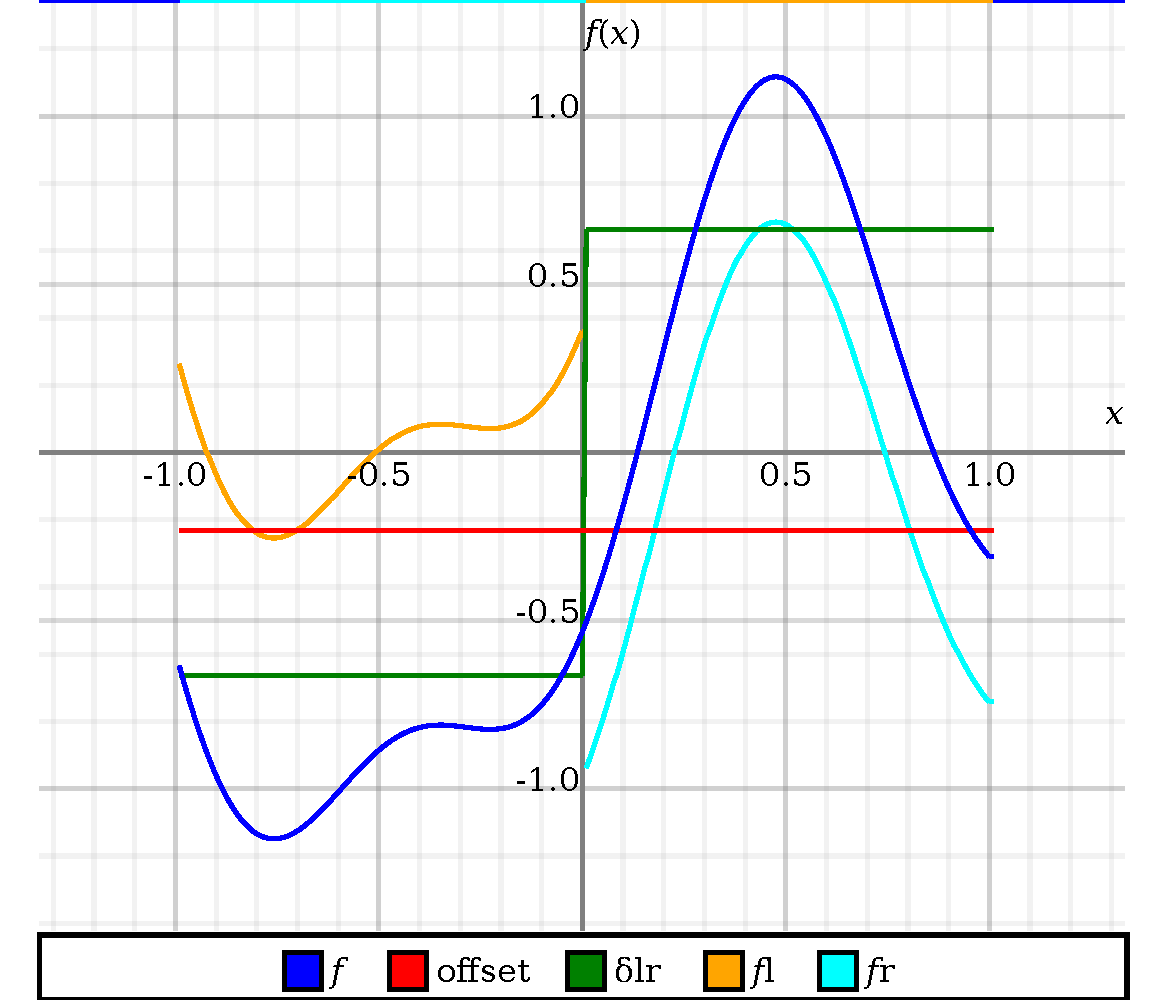
\includegraphics[width=\linewidth]{Haar-domDecompose.pdf}
 \caption{Example of how a function $f:D^1\to\mathbb{R}$ is decomposed into a constant offset, plus a step-function (Haar wavelet) for the offset-difference between left and right half, plus local fluctuations in each of the halves.}
 \label{haarDomDecompose}
\end{figure}
To still support functions with nonzero integral, one can simply add an absolute offset with a wrapper-type only at the top level:
\begin{lstlisting}
data Haar_D¹ dn y = Haar_D¹
    { global_offset :: !y
    , variation :: HaarUnbiased y }
\end{lstlisting}
The name “Haar” indicates that the basis functions of this data type (meaning those functions represented when exactly one of the fields of type ℝ in the \lstinline`HaarUnbiased ℝ` structure is 1, all other zero) are exactly the unnormalised Haar wavelets.

%% Acknowledgments
\begin{acks}                            %% acks environment is optional
                                        %% contents suppressed with 'anonymous'
  %% Commands \grantsponsor{<sponsorID>}{<name>}{<url>} and
  %% \grantnum[<url>]{<sponsorID>}{<number>} should be used to
  %% acknowledge financial support and will be used by metadata
  %% extraction tools.
  This material is based upon work supported by the
  \grantsponsor{GS100000001}{National Science
    Foundation}{http://dx.doi.org/10.13039/100000001} under Grant
  No.~\grantnum{GS100000001}{nnnnnnn} and Grant
  No.~\grantnum{GS100000001}{mmmmmmm}.  Any opinions, findings, and
  conclusions or recommendations expressed in this material are those
  of the author and do not necessarily reflect the views of the
  National Science Foundation.
\end{acks}


%% Bibliography
%\bibliography{bibfile}


%% Appendix
\appendix
\section{Appendix}

Text of appendix \ldots

\end{document}
